\chapter{Interior Point Method}
Interior point methods are modified versions of Newtons method for bound, constrained problems, where the algorithm at each iteration satisfies the constraints strictly. Thus, the methods approach the solution from within the feasible region, thus giving rise to their name. The interior point methods provide efficient performance while having better theoretical properties than the standard simplex method.\\

A general bound, constrained minimization problem can be stated as
\begin{align*}
	\min_{x \in \mathbb{R}^n} \;  & \; f(x) \\
	\text{subject to} \;  & \; c_i(x) = 0 \; , \qquad i \in \mathcal{E} \\
							& \; c_i(x) \geq 0  \; , \qquad  i \in \mathcal{I} \\
							& \; x \geq 0
\end{align*}
where $E$ and $I$ is the set of equalities and inequalities respectively, and $f \; . \; \mathbb{R}^n \to \mathbb{R}$.
In practice working with equality constraints is often easier. Hence, the inequality constraint are often turned into equality constraints through the use of \textit{slack variables}, which make up the difference between the left and right side \cite{ipopt}. Thus, transforming the inequality $A x \leq b$ into
\begin{align*}
	A x + u &= b \\
	u & \geq 0 \; .
\end{align*}
Although this does introduce the additional variable $u$, having only equality conditions for boundaries is generally easier to work with.

\section{Karush–Kuhn–Tucker Conditions}
A central theorem in mathematical optimization are the Karush–Kuhn–Tucker conditions, or KKT conditions, which are first-order conditions for for a solution of a nonlinear problem to be an optimum. The KKT conditions allow inequality constraints, thus being more general than Lagrange multipliers, which only allow equalities. The KKT conditions can be stated as follows \cite{wright}
\begin{theorem}
	Suppose that $x^*$ is a local solution of the objective function $f \; . \; \mathbb{R}^n \to \mathbb{R}$ with respect to a collection of constraints $\{ c_i(x) \in \mathcal{E} \vee c_i(x) \in \mathcal{I} \}_{i=1}^{m}$, where $c_i \; . \; \mathbb{R}^n \to \mathbb{R}$. Let $\mathcal{L}$ be the Lagrangian of the problem. If the subset of the constraints $\{ c_i(x) \in \mathcal{E}\}$ has the property that $\{ \nabla c_i(x^*)\}$ is linear independent, then there is a vector of Lagrange multipliers, $\lambda^*$, for which the following holds:
	\begin{subequations}	
	\begin{align}
		\nabla_x \mathcal{L}(x^*,\lambda^*) &= 0 \; ,  \\
		c_i(x^*) &= 0 \; , \qquad \forall i \in \mathcal{E} \\
		c_i(x^*) &= 0 \; , \qquad \forall i \in \mathcal{I} \\
		\lambda_{i}^* &\geq 0 \; , \qquad \forall i \in \mathcal{I} \\
		\lambda_{i}^* c_i(x^*) &= 0 \; , \qquad \forall i \in \mathcal{E} \cup \mathcal{I}
	\end{align}
	\end{subequations}	  
\end{theorem}
The KKT conditions is a way of determining whether a point is an optimum, since if $x^*$ satisfies the conditions, then its objective value must be lower than the objective point of any other point.
Note, that for $m = 0$ the set $\mathcal{I}$ is empty, thus only equality conditions are present, and $\lambda$ becomes regular Lagrange multipliers. 

\section{Duality Theory}
Consider a minimization problem such as the linear problem
\begin{align*}
	\min_{x \in \mathbb{R}^n} \;  & \; c^T x \\
	\text{subject to} \;  & \; A x = b  \\
							& \; x \geq 0 \; ,
\end{align*}
which will be denoted as the \textit{primal} problem. The \textit{dual} to this problem is defined as 
\begin{align*}
	\max_{\lambda \in \mathbb{R}^n} \;  & \; b^T \lambda \\
	\text{subject to} \;  & \; A^T \lambda + s = c  \\
							& \; s \geq 0 \; .
\end{align*}
This is another linear optimum problem with the unique property, that the Lagrange multipliers of the primal problem are the optimal variables of the dual problem and vice versa. Thus, the dual problem allows a lot of information to be obtained about the primal problem. Note, that the dual problem of the dual is nothing but the initial primal problem.
An important property of the dual problem is, that it has the exact same KKT conditions as the primal, thus prompting the following theorem \cite{wright}:
\begin{theorem}
If either the primal or the dual problem has a solution, then so does the other, and the objective values are equal. If either problem is unbounded, then the other problem is infeasible. If a solution exists, then the optimal solution to the dual problem are the Lagrange multipliers to the primal problem and vice versa.
\end{theorem}

Therefore, for primal-dual algorithms one utilizes a triplet of variables $(x , \lambda , s)$ when computing the optimum of a function.

\section{Barrier Problems}
In interior point methods the boundaries of the variables are enforced through a barrier function, which keeps the objective function continuously differentiable.
Consider the same standard linear optimization problem as earlier. To this problem one can associate a \textit{barrier function}, $B(x , \mu)$, defined as
\begin{equation}
	B(x , \mu) = c^T x - \mu \sum_{i=1}^{n} \ln x_i \; ,
\end{equation} 
where the barrier parameter $\mu > 0$ determines how "sharp" the boundary of the parameter is, as seen in figure \ref{fig:barrier}. Note, how for $\mu \to 0$ one recovers the original problem.
\begin{figure}[h!]
	\centering
	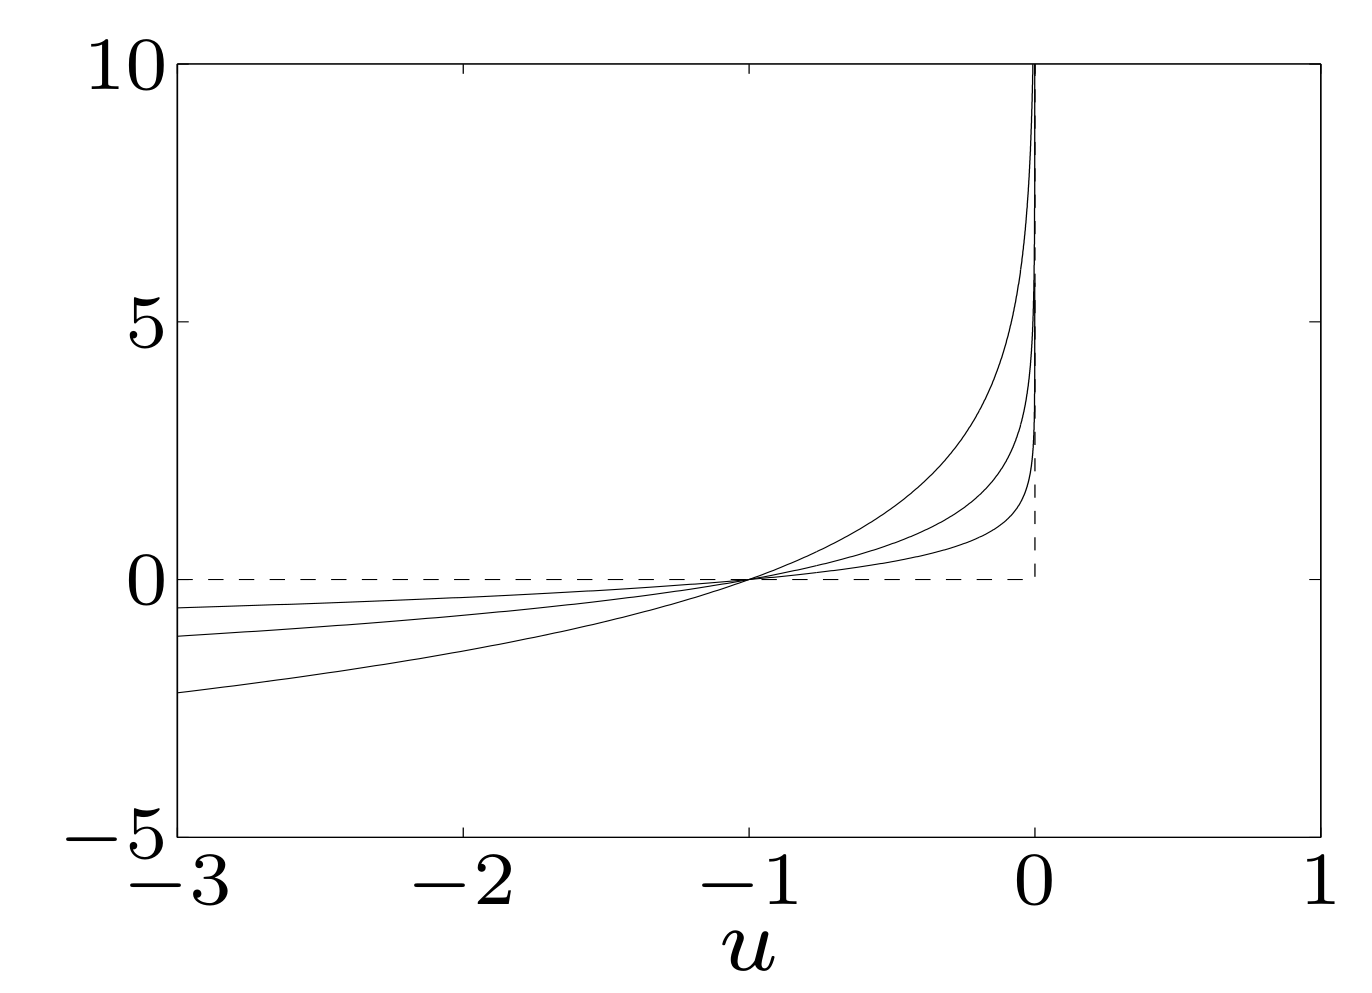
\includegraphics[width=0.6\textwidth]{Figures/barrier.png}
	\caption{\textit{Barrier term for various $\mu$ (here $u$). At $\mu \to 0$ the barrier turns into the strict inequality constraint of the original problem.}}
	\label{fig:barrier}
\end{figure}
Instead of minimizing the old problem, it is now of interest of solving the barrier problem 
\begin{align*}
	\min_{x \in \mathbb{R}^n} \;  & \; B(x , \mu) \\
	\text{subject to} \;  & \; A x = b   \; ,
\end{align*}
where the constraint on $x$ no longer is needed due to the barrier. Associated to the new barrier problem is the Lagrangian
\begin{equation}
	\mathcal{L}(x, \lambda, s) = c^T x - \mu \sum_{i=1}^{n} \ln x_i - \lambda^T (A x -b) \; ,
\end{equation}
where $\lambda \in \mathbb{R}^m$ is the Lagrange multiplier for the $A x = b$ constraint. Now let $X = \mathrm{Diag}(x_1 , \ldots , x_n)$, $e = (1,1, \ldots , 1)^T$, $s = \mu X^{-1} e$, and $S = \mathrm{Diag}(s_1 , \ldots , s_n)$. Using these one can state the KKT conditions of the barrier problem as 
\begin{subequations}
\begin{align}
	A^T \lambda + s &= c \\
	A x &= b \\
	X S e &= \mu e \; .
\end{align}
\end{subequations}
Comparing these to the KKT conditions of the original problem
\begin{subequations}
\begin{align}
	A^T \lambda + s &= c \\
	A x &= b \\
	x_i s_i &= 0 \; \text{for } i = 1, \ldots , n  \; ,
\end{align}
\end{subequations}
one can easily see that the $\mu$ of the barrier function has "relaxed" the KKT complementary condition \cite{ipnote}. Again, for $\mu \to 0$ one returns to the original problem. 


\section{Primal-Dual Interior Point Method}
By considering the previously explained concepts, one can alter the classical Newton's method to take into account the constraints of the problem, such that one can compute a constrained Newton step, which allows iteration of the parameters towards the optimum.
By solving the \textit{barrier subproblem} for a given $\mu$, one will find the optimum solution of said subproblem. Thus, solving these subproblems iteratively for ever decreasing $\mu$ using the previous solution as starting point, one will approach the optimal solution of the original problem $x^*$ as $\mu \to 0$ \cite{ipopt}.\\
In the linear case the Primal-Dual Interior Point Method solves two problems  simultaneously:\\
\textbf{Primal:}
 \begin{align*}
	\min_{x \in \mathbb{R}^n} \;  & \; c^T x \\
	\text{subject to} \;  & \; A x = b  \\
							& \; x \geq 0 \; ,
\end{align*}
\textbf{Dual:} 
\begin{align*}
	\max_{\lambda \in \mathbb{R}^n} \;  & \; b^T \lambda \\
	\text{subject to} \;  & \; A^T \lambda + s = c  \\
							& \; s \geq 0 \; .
\end{align*}
The solutions for these problems are characterized by the same KKT conditions, which were listed earlier. These conditions can be written into a single mapping
 \begin{align}
    F(x , \lambda, s) &= \begin{pmatrix}
           A^T \lambda + s - c \\
           A x - b \\
           X S e
         \end{pmatrix} = 0
  \end{align}
  which has the Jacobian
 \begin{align}
    J(x , \lambda, s) = \begin{pmatrix}
           0 & A^T & I	\\
           A & 0 & 0 	\\
           S & 0 & X
         \end{pmatrix}
  \end{align}
Thus, one can write the Newton direction $(x_B , \lambda_B , s_B)$ as the solution to the system of equations
\begin{align}
J \begin{pmatrix}
           x_B \\
           \lambda_B \\
           s_B
         \end{pmatrix} = -F
\end{align}
This equation does not take into account the barrier function, however, as stated earlier, the effect of the barrier term is to relax the the KKT complementary condition. Thus, by setting $X S e = \mu e$ one obtains
\begin{align}
	\begin{pmatrix}
    	 0 & A^T & I    \\
         A & 0 & 0 		\\
         S & 0 & X
    \end{pmatrix} 
    \begin{pmatrix}
    	x_b 		    \\
        \lambda_B		\\
        s_B
    \end{pmatrix} =
    - \begin{pmatrix}
    	  A^T \lambda + s - c 	\\
          A x - b 				\\
          X S e - \mu e
    \end{pmatrix} \; . \label{eq:newtondirection}
\end{align}
Thus, one can iteratively update the parameters in the algorithm using the Newton calculated Newton direction
\begin{equation}
	(x_{k+1} , \lambda_{k+1} , s _{k+1}) = (x_{k} , \lambda_{k} , s _{k}) + \alpha  (x_B , \lambda_B , s_B) \; , \label{eq:newtonstep}
\end{equation}
where $alpha$ can be found using a line-search or other more sophisticated methods.
The procedure above can be summarized in the following algorithm \cite{ipnote}:\\
\begin{algorithmic}
\State Choose $\sigma \in (0,1)$ and $\mu_0 > 0$.
\State Choose point $(x_0 , \lambda_0 , s_0)$ within feasible region.
\For{$k = 1 , \ldots$}
	\State $\mu_k \gets \sigma \mu_{k-1}$
	\State Calculate the Newton direction using equation \ref{eq:newtondirection}.
	\State Find $\alpha$.
	\State $x_{k+1} \gets \alpha p_b$
\EndFor
\end{algorithmic}
The name of the method should now be easily understood, as the methods starts in the interior of the feasible region and works it way towards the boundary. The path that the algorithm traces out through the feasible region is called the \textit{central path} and can be used for proving the convergence of the algorithm \cite{wright}.
